\documentclass[12pt]{article}
\usepackage{graphicx}
\usepackage{amsmath}   
\usepackage{commath}
\usepackage{gensymb}
\usepackage{graphicx}


\begin{document}
\title{\textbf{Triangles}}
\maketitle
\begin{center}
\end{center}

\begin{enumerate}
\section*{9$^{th}$ Maths - Chapter 7}

\item In an isosceles triangle $ABC$, with $AB = AC$, the bisectors of $\angle$ B and $\angle$ C intersect each other at O. Join A to O. Show that :
\begin{enumerate}
$OB = OC$  $AO$ bisects $\angle$ A
\end{enumerate}
\item In $\triangle$ ABC, $AD$ is the perpendicular bisector of $BC$.Show that $\triangle$ABC an isosceles triangle in which $AB = AC$.
\begin{figure}[!h]
\begin{center}
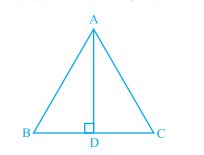
\includegraphics[width=\columnwidth]{./figs/triangle2.png}
\end{center}                                      \caption{}                                        \label{fig:Fig1}                                  \end{figure}
\item $ABC$ is an isosceles triangle in which altitudes $BE$ and $CF $are drawn to equal sides $AC $and $AB$respectively. Show that these altitudes are equal.
\begin{figure}[!h]
\begin{center}
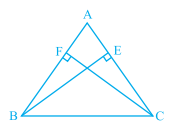
\includegraphics[width=\columnwidth]{./figs/triangle3.png}
 \end{center}
	\caption{}
\label{fig:Fig1}
\end{figure}
\item $ABC$ is a triangle in which altitudes $BE$ and $CF$ to sides $AC $and $AB$ are equal. Show that 
\item $\triangle$ABE $\cong$  $\triangle$ ACF
\item $AB = AC$, i.e.,$ABC$is an isosceles triangle
\begin{figure}[!h]
\begin{center}
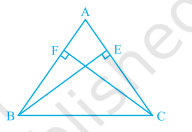
\includegraphics[width=\columnwidth]{./figs/triangle4.png}
\end{center}
	\caption{}                                     
\label{fig:Fig1}
\end{figure}
\item $ABC$and $DBC$ are two isosceles triangles on the same base $BC$. Show that
$\angle$ABD = $\angle$ACD.
\begin{figure}[!h]
\begin{center}
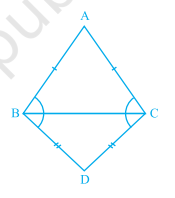
\includegraphics[width=\columnwidth]{./figs/triangle6.png}
\end{center}                                      \caption{}                                        \label{fig:Fig1}                                  \end{figure}
\item$\triangle$ABC is an isosceles triangle in which $AB = AC$.Side $BA $is produced to $D$ such that$ AD = AB$.Show that $\angle$BCD is a right angle.
	\begin{figure}[!h]
\begin{center}
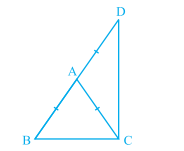
\includegraphics[width=\columnwidth]{./figs/triangle7.png}
\end{center}                                      \caption{}                                        \label{fig:Fig1}                                  \end{figure}
\item $ABC$is a right angled triangle in which $\angle$A = 90\degree and $AB = AC$. Find $\angle$Band $\angle$C.
\item Show that the angles of an equilateral triangle are 60\degree each.
\end{enumerate}
\end{document}
